\documentclass[aspectratio=1610,onlymath, ngerman]{beamer}
% \documentclass[aspectratio=1610,onlymath,handout]{beamer}
\usepackage[ngerman]{babel}
\usepackage[utf8]{inputenc}
\usepackage[T1]{fontenc}

\usetheme[nosectionnum,pagenum,sansmath, cd2018, nodin]{tud}

%\usefonttheme[onlymath]{serif}
\usepackage{opensans}
\usepackage{stmaryrd}
\usepackage[normalem]{ulem} % sout command
\usepackage{txfonts}
\DeclareMathAlphabet{\mathsc}{OT1}{cmr}{m}{sc}

\usepackage{listings}
\lstset{language=Haskell,basicstyle=\ttfamily}
\usepackage{verbatim}
\usepackage{bold-extra}

\setbeamerfont{title}{size=\Huge, family=\bfseries\fosfamily}
\setbeamerfont{frametitle}{size=\LARGE, family=\bfseries\fosfamily}

\setbeamerfont{normal text}{size=\normalsize}
\setbeamerfont{itemize/enumerate body}{}
\setbeamerfont{itemize/enumerate subbody}{size=\small}
\setbeamerfont{itemize/enumerate subsubbody}{size=\footnotesize}

\usepackage{tudscrcolor}
\usepackage{environ}
\usepackage{tikz}
\usetikzlibrary{arrows,positioning,decorations.pathreplacing}
% Inspired by http://www.texample.net/tikz/examples/hand-drawn-lines/
\usetikzlibrary{decorations.pathmorphing}
\pgfdeclaredecoration{penciline}{initial}{
    \state{initial}[width=+\pgfdecoratedinputsegmentremainingdistance,
    auto corner on length=1mm,]{
        \pgfpathcurveto%
        {% From
            \pgfqpoint{\pgfdecoratedinputsegmentremainingdistance}
            {\pgfdecorationsegmentamplitude}
        }
        {%  Control 1
            \pgfmathrand
            \pgfpointadd{\pgfqpoint{\pgfdecoratedinputsegmentremainingdistance}{0pt}}
            {\pgfqpoint{-\pgfdecorationsegmentaspect
                    \pgfdecoratedinputsegmentremainingdistance}%
                {\pgfmathresult\pgfdecorationsegmentamplitude}
            }
        }
        {%TO
            \pgfpointadd{\pgfpointdecoratedinputsegmentlast}{\pgfpoint{1pt}{1pt}}
        }
    }
    \state{final}{}
}
\tikzset{handdrawn/.style={decorate,decoration=penciline}}
\tikzset{every shadow/.style={fill=none,shadow xshift=0pt,shadow yshift=0pt}}

\NewEnviron{doodlebox}[2]{%
    \begin{tikzpicture}[decoration=penciline, decorate]%
    \pgfmathsetseed{1237}%
    \node (n1) [decorate,draw=#1, fill=#2,thick,align=justify, text width=0.97\textwidth, inner ysep=2mm, inner xsep=2mm] at (0,0) {\BODY};%
    \end{tikzpicture}%
}
\NewEnviron{doodle}[1]{%
    \begin{tikzpicture}[decoration=penciline, decorate]%
    \pgfmathsetseed{1237}%
    \node (n1) [decorate,draw=#1, fill=#1!10,thick,align=justify, text width=0.97\textwidth, inner ysep=2mm, inner xsep=2mm] at (0,0) {\BODY};%
    \end{tikzpicture}%
}

\newcommand{\defineTitle}[3]{%
    \newcommand{\lectureindex}{#1}%
    \title{Programmierung}%
    \subtitle{Übung #1: #2}%
    \author{Eric Kunze \\ \url{eric.kunze@mailbox.tu-dresden.de} }%
    \date{#3}%
    \datecity{TU Dresden}%
}

%%%%%%%%%%%%%%%%%%%%%%%%%%%%%%%%%%%%%%%%%%%%%%%%%%%%%%%%%%%%%%%%%%%%%%%%%%%%
%%%%%%%%%%%%%%%%%%%%%%%%%%%%%%%%%%%%%%%%%%%%%%%%%%%%%%%%%%%%%%%%%%%%%%%%%%%%

\defineTitle{10}{$C_0$ und $AM_0$}{21.~Juni~2019}

\usepackage[inline]{enumitem}

\renewcommand{\emph}[1]{\textbf{#1}}
\newcommand{\coloremph}[1]{\textcolor{cdpurple}{#1}}
\newcommand{\col}[1]{\textcolor{cdpurple}{\boldsymbol{#1}}}
\newcommand{\coll}[1]{\textcolor{cddarkgreen}{\boldsymbol{#1}}}
\newcommand{\colll}[1]{\textcolor{cdorange}{\boldsymbol{#1}}}

\DeclareMathSymbol{*}{\mathbin}{symbols}{"01}

\renewcommand*{\headerinfo}{\color{cdgray}\textbf{Github:} \url{https://github.com/oakoneric/programmierung-ss19}}
\arraycolsep2pt

\usepackage{aligned-overset}
\usepackage{array}
\chardef\_=`_

\renewcommand{\epsilon}{\varepsilon}
\newcommand{\labelitemi}{$\blacktriangleright$}
\newcommand{\labelitemii}{$\vartriangleright$}

\begin{document}
    \maketitle
    
    \begin{frame} \frametitle{$C_0$ und $AM_0$}
    \small
    	\begin{itemize}
    		\item \emph{Ziel:} Implementierung einer einfachen Programmiersprache $C_1$
    		\item \emph{Hier:} zunächste Einschränkung auf $C_0$ \pause
    			\begin{itemize}
    				\item genau eine main-Funktion
    				\item Zugriff auf \texttt{stdio} durch \texttt{\# include}
    				\item einzig zugelassende Datenstruktur: \texttt{int}, Konstanten
    				\item Kontrollstrukturen: Ein-/Ausgabebefehle, Zuweisungen, Sequenzen, Verzweigungen, bedingte Schleifen
    			\end{itemize}
    		\pause
    		\item \emph{Implementierung} durch
    			\begin{itemize}
    				\item Syntax von $C_0$
    				\item Befehle und Semantik einer abstrakten Maschine $AM_0$
    				\item Übersetzer $C_0 \leftrightarrow AM_0$
    			\end{itemize}
    	\end{itemize}
    \end{frame}

	\begin{frame} \frametitle{Übersetzung von \texttt{if - then - else}}
	\small \centering
	\begin{align*}
		sttrans( \texttt{if (} &exp \texttt{)} \ stat_1 \ \texttt{else} \ stat_2, tab, a) := \\
		& boolexptrans(exp, tab) \\
		&\texttt{JMC} \ a.1 ; \\
		& sttrans(stat_1, tab, a.2) \\
		&\texttt{JMP} \ a.3; \\
		a.1: \quad & sttrans(stat_2, tab, a.4) \\
		a.3: \quad & \phantom{.}
	\end{align*}
	für alle $exp \in \mathrm{W}(\langle \mathrm{BoolExpression} \rangle )$, $stat_1, stat_2 \in \mathrm{W}(\langle \mathrm{Statement} \rangle )$, $tab \in \mathrm{Tab}$ und $a \in \mathbb{N}^\ast$.
%		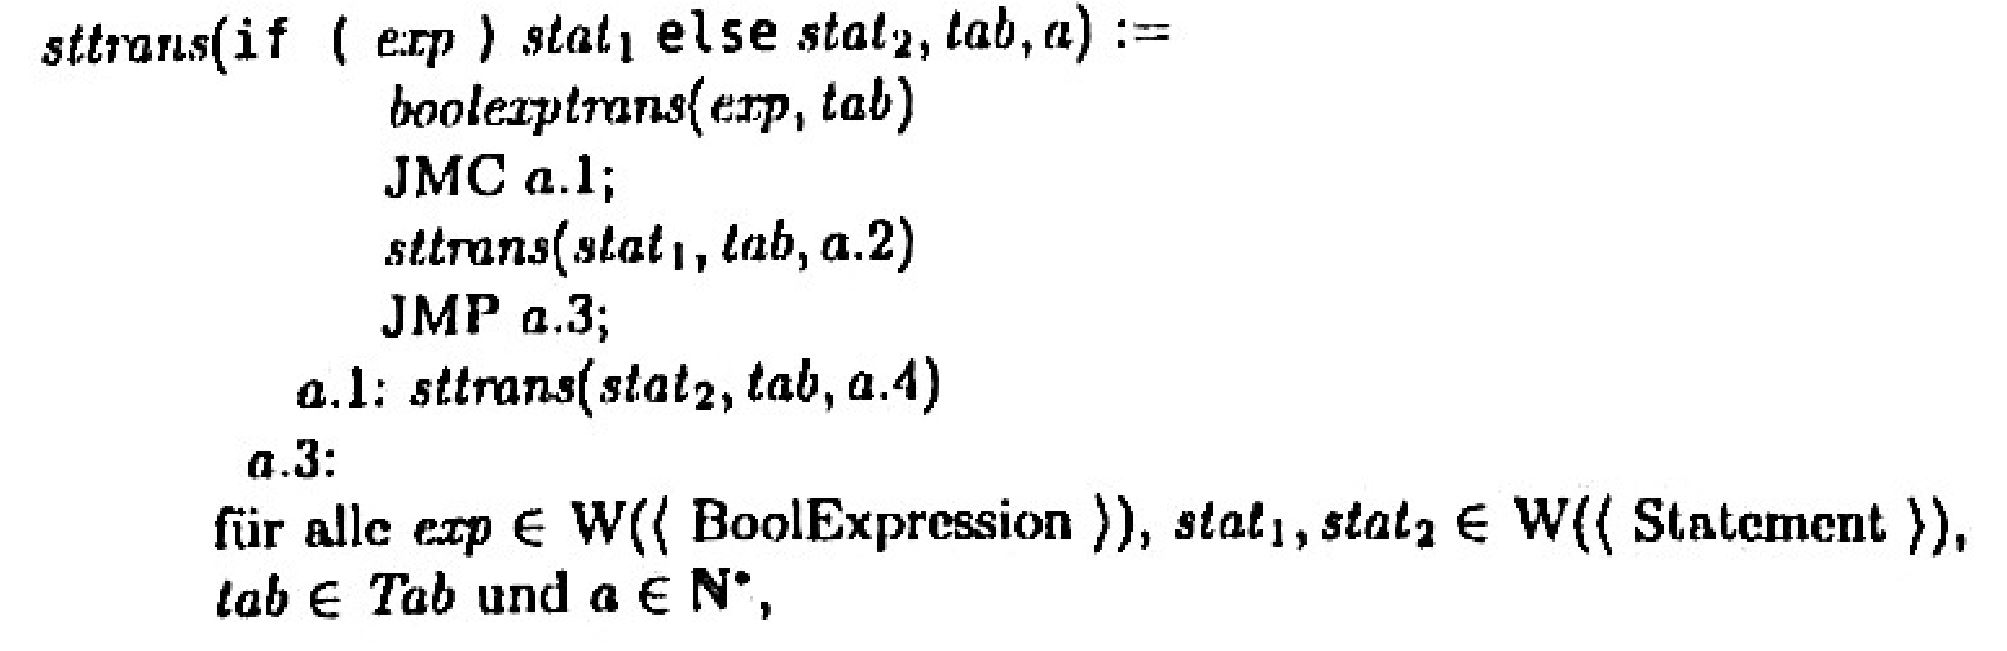
\includegraphics[width=\linewidth]{C0_trans_if.jpg}	
	\end{frame}


	\begin{frame}<handout:0> \frametitle{Aufgabe 1}
	\small
		\begin{minipage}{\dimexpr0.5\linewidth-\fboxrule-\fboxsep}
			\begin{ttfamily}
				\begin{enumerate}[label=\arabic* $\enskip$, nolistsep]
					\item \#\!\!\! include <stdio.h>
					\item \emph{int} main( ) \{
					\item $\quad$ \emph{int} a,b,max;
					\item $\quad$ scanf("\%i", \&a);
					\item $\quad$ scanf("\%i", \&a);
				\end{enumerate}
			\end{ttfamily}
		\end{minipage}
		\begin{minipage}{\dimexpr0.5\linewidth-\fboxrule-\fboxsep}
			\begin{ttfamily}
				\begin{enumerate}[label=\arabic* $\enskip$, nolistsep]
					\setcounter{enumi}{5}
					\item $\quad$ \emph{if} (a > b) max = a;
					\item $\quad$ \emph{else} max = b;
					\item $\quad$ printf("\%d", max);
					\item $\quad$ \emph{return} 0;
					\item \}
				\end{enumerate}
			\end{ttfamily}
		\end{minipage}
	\end{frame}
    
    \begin{frame} \frametitle{Aufgabe 1 -- Teil (a)}
    \small
	    \begin{minipage}{\dimexpr0.5\linewidth-\fboxrule-\fboxsep}
	    	\emph{Baumstrukturierte Adressen:} \\
	    	
	    	\begin{tabular}{>{\ttfamily}r >{\ttfamily}l}
	                       & READ 1; \\
	    			       & READ 2; \\
	    			       & LOAD 1; \\
	    			       & LOAD 2; \\
	    			       & GT; \\
	    		           & JMC 1.3.1; \\
	    			       & LOAD 1; \\
	    			       & STORE 3; \\
	    			       & JMP 1.3.3; \\
	    			1.3.1: & LOAD 2; \\
	    			       & STORE 3; \\
	    			1.3.3: & WRITE 3; 
	    	\end{tabular}
	    \end{minipage}
    	\pause
	    \begin{minipage}{\dimexpr0.5\linewidth-\fboxrule-\fboxsep}
	    	\emph{Linearisierte Adressen:} \\
	    	
	    	\begin{tabular}{>{\ttfamily}r >{\ttfamily}l}
	    			1: & READ 1; \\
	    			2: & READ 2; \\
	    			3: & LOAD 1; \\
	    			4: & LOAD 2; \\
	    			5: & GT; \\
	    			6: & JMC 10; \\
	    			7: & LOAD 1; \\
	    			8: & STORE 3; \\
	    			9: & JMP 12; \\
	    			10: & LOAD 2; \\
	    			11: & STORE 3; \\
	    			12: & WRITE 3; 
	    	\end{tabular}
	    \end{minipage}
    \end{frame}
    
    \begin{frame} \frametitle{Aufgabe 1 -- Teil (b)}
    \small
    		\emph{Ablauf der abstrakten Maschine:} 
    		\begin{center}
    			\begin{tabular}{rrcrclcrcrl}
    				& BZ &,& DK &,& HS &,& Inp &,& Out & \\
    				( & 1 &,& $\epsilon$ &,& [ ] &,& 5:7 &,& $\epsilon$ & ) \\
    				( & 2 &,& $\epsilon$ &,& [1/5] &,& 7 &,& $\epsilon$ & ) \\
    				( & 3 &,& $\epsilon$ &,& [1/5, 2/7] &,& $\epsilon$ &,& $\epsilon$ & ) \\
    				( & 4 &,& 5 &,& [1/5, 2/7] &,& $\epsilon$ &,& $\epsilon$ & ) \\
    				( & 5 &,& 7:5 &,& [1/5, 2/7] &,& $\epsilon$ &,& $\epsilon$ & ) \\
    				( & 6 &,& 0 &,& [1/5, 2/7] &,& $\epsilon$ &,& $\epsilon$ & ) \\
    				( & 10 &,& $\epsilon$ &,& [1/5, 2/7] &,& $\epsilon$ &,& $\epsilon$ & ) \\
    				( & 11 &,& 7 &,& [1/5, 2/7 ] &,& $\epsilon$ &,& $\epsilon$ & ) \\
    				( & 12 &,& $\epsilon$ &,& [1/5, 2/7, 3/7] &,& $\epsilon$ &,& $\epsilon$ & ) \\
    				( & 13 &,& $\epsilon$ &,& [1/5, 2/7, 3/7] &,& $\epsilon$ &,& 7 & ) \\
    			\end{tabular}
    		\end{center}
    		
    		\pause   		

    		\begin{equation*}
    		\mathcal{P} [\![ Max_0 ]\!] (5:7) = proj_5^{(5)} \Bigl( \mathcal{I}[\![ Max_0 ]\!] (1,\epsilon, [],5:7,\epsilon) \Bigr) = 7
    		\end{equation*}
    \end{frame}

	\begin{frame}<handout:0> \frametitle{Aufgabe 2}
	\small
		\begin{minipage}{\dimexpr0.5\linewidth-\fboxrule-\fboxsep}
			\begin{ttfamily}
				\begin{enumerate}[label=\arabic* $\enskip$, nolistsep]
					\item \#\!\!\! include <stdio.h>
					\item 
					\item \emph{int} main( ) \{
					\item $\quad$ \emph{int} x,y,a;
					\item $\quad$ scanf("\%i", \&y);
					\item $\quad$ scanf("\%i", \&a);
					\item x = 0;
				\end{enumerate}
			\end{ttfamily}
		\end{minipage}
		\begin{minipage}{\dimexpr0.5\linewidth-\fboxrule-\fboxsep}
			\begin{ttfamily}
				\begin{enumerate}[label=\arabic* $\enskip$, nolistsep]
					\setcounter{enumi}{7}
					\item $\quad$ \emph{while} (x < a) \{
					\item $\quad$ $\quad$ x = x + 1;
					\item $\quad$ $\quad$ y = y * y;
					\item $\quad$ \}
					\item $\quad$ printf("\%d", y);
					\item $\quad$ \emph{return} 0;
					\item \}
				\end{enumerate}
			\end{ttfamily}
		\end{minipage}
	\end{frame}
	
    \begin{frame} \frametitle{Aufgabe 2 -- Teil (a)}
    \small
    \centering
	    \begin{minipage}{\dimexpr0.3\linewidth-\fboxrule-\fboxsep}
	    	\centering
	    	\begin{ttfamily}
	    		\begin{enumerate}[label=\arabic*:, nolistsep, leftmargin=*]
	    			\item READ 2; 
	    			\item READ 3;
	    			\item LIT 0;
	    			\item STORE 1;
	    			\item LOAD 1;
	    			\item LOAD 3;
	    			\item LT;
	    			\item JMC 18;
	    			\item LOAD 1;
	    		\end{enumerate}
	    	\end{ttfamily}
	   \end{minipage}
	   \begin{minipage}{\dimexpr0.3\linewidth-\fboxrule-\fboxsep}
	   	\centering
	    	\begin{ttfamily}
	    		\begin{enumerate}[label=\arabic*:, nolistsep, leftmargin=*]
	    			\setcounter{enumi}{9}
	    			\item LIT 1;
	    			\item ADD; 
	    			\item STORE 1;
	    			\item LOAD 2;
	    			\item LOAD 2; 
	    			\item MUL;
	    			\item STORE 2;
	    			\item JMP 5;
	    			\item WRITE 2;
	    		\end{enumerate}
	    	\end{ttfamily}
	    \end{minipage}
    \end{frame}

	\begin{frame}<handout:0> \frametitle{Aufgabe 2}
	\small
		\begin{minipage}{\dimexpr0.33\linewidth-\fboxrule-\fboxsep}
			\begin{ttfamily}
				\begin{enumerate}[label=\arabic*:, nolistsep, leftmargin=*]
					\item READ 1;
					\item READ 2; 
					\item LOAD 1;
				\end{enumerate}
			\end{ttfamily}
		\end{minipage}
		\begin{minipage}{\dimexpr0.33\linewidth-\fboxrule-\fboxsep}
			\begin{ttfamily}
				\begin{enumerate}[label=\arabic*:, nolistsep, leftmargin=*]
					\setcounter{enumi}{3}
					\item LOAD 2;
					\item LIT 0; 
					\item SUB;
				\end{enumerate}
			\end{ttfamily}
		\end{minipage}
		\begin{minipage}{\dimexpr0.33\linewidth-\fboxrule-\fboxsep}
			\begin{ttfamily}
				\begin{enumerate}[label=\arabic*:, nolistsep, leftmargin=*]
					\setcounter{enumi}{6}
					\item JMC 9;
					\item JMP 5; 
					\item WRITE 2;
				\end{enumerate}
			\end{ttfamily}
		\end{minipage}
	\end{frame}

	\begin{frame}<handout:0> \frametitle{Aufgabe 2 -- Teil (b)}
	\small
		\begin{center}
			\begin{tabular}{rrcrclcrcrl}
				& BZ &,& DK &,& HS &,& Inp &,& Out & \\
				( & 1 &,& $\epsilon$ &,& [ ] &,& 0:1 &,& $\epsilon$ & ) \\
				( & 2 &,& $\epsilon$ &,& [1/0] &,& 1 &,& $\epsilon$ & ) \\
				( & 3 &,& $\epsilon$ &,& [1/0, 2/1] &,& $\epsilon$ &,& $\epsilon$ & ) \\
				( & 4 &,& 0 &,& [1/0, 2/1] &,& $\epsilon$ &,& $\epsilon$ & ) \\
				( & 5 &,& 1:0 &,& [1/0, 2/1] &,& $\epsilon$ &,& $\epsilon$ & ) \\
				( & 6 &,& 0:1:0 &,& [1/0, 2/1] &,& $\epsilon$ &,& $\epsilon$ & ) \\
				( & 7 &,& 1:0 &,& [1/0, 2/1] &,& $\epsilon$ &,& $\epsilon$ & ) \\
				( & 8 &,& 0 &,& [1/0, 2/1] &,& $\epsilon$ &,& $\epsilon$ & ) \\
				( & 5 &,& 0 &,& [1/0, 2/1] &,& $\epsilon$ &,& $\epsilon$ & ) \\
				( & 6 &,& 0:0 &,& [1/0, 2/1] &,& $\epsilon$ &,& $\epsilon$ & ) \\
				( & 7 &,& 0 &,& [1/0, 2/1] &,& $\epsilon$ &,& $\epsilon$ & ) \\
				( & 9 &,& $\epsilon$ &,& [1/0, 2/1] &,& $\epsilon$ &,& $\epsilon$ & ) \\
				( & 10 &,& $\epsilon$ &,& [1/0, 2/1] &,& $\epsilon$ &,& 1 & ) \\
			\end{tabular}
		\end{center}
	\end{frame}
    
    \newcommand{\cw}[1]{\textcolor{cdgray!50}{#1}}
    \begin{frame} \frametitle{Aufgabe 2 -- Teil (b)}
    \small
	    \begin{center}
	    	\begin{tabular}{rrcrclcrcrl}
	    		& BZ &,& DK &,& HS &,& Inp &,& Out & \\
	    		( & 1 &,& $\epsilon$ &,& [ ] &,& 0:1 &,& $\epsilon$ & ) \\
	    		( & 2 &,& \cw{$\epsilon$} &,& [1/0] &,& 1 &,& \cw{$\epsilon$} & ) \\
	    		( & 3 &,& \cw{$\epsilon$} &,& [1/0, 2/1] &,& $\epsilon$ &,& \cw{$\epsilon$} & ) \\
	    		( & 4 &,& 0 &,& \cw{[1/0, 2/1]} &,& \cw{$\epsilon$} &,& \cw{$\epsilon$} & ) \\
	    		( & 5 &,& 1:0 &,& \cw{[1/0, 2/1]} &,& \cw{$\epsilon$} &,& \cw{$\epsilon$} & ) \\
	    		( & 6 &,& 0:1:0 &,& \cw{[1/0, 2/1]} &,& \cw{$\epsilon$} &,& \cw{$\epsilon$} & ) \\
	    		( & 7 &,& 1:0 &,& \cw{[1/0, 2/1]} &,& \cw{$\epsilon$} &,& \cw{$\epsilon$} & ) \\
	    		( & 8 &,& 0 &,& \cw{[1/0, 2/1]} &,& \cw{$\epsilon$} &,& \cw{$\epsilon$} & ) \\
	    		( & 5 &,& \cw{0} &,& \cw{[1/0, 2/1]} &,& \cw{$\epsilon$} &,& \cw{$\epsilon$} & ) \\
	    		( & 6 &,& 0:0 &,& \cw{[1/0, 2/1]} &,& \cw{$\epsilon$} &,& \cw{$\epsilon$} & ) \\
	    		( & 7 &,& 0 &,& \cw{[1/0, 2/1]} &,& \cw{$\epsilon$} &,& \cw{$\epsilon$} & ) \\
	    		( & 9 &,& $\epsilon$ &,& \cw{[1/0, 2/1]} &,& \cw{$\epsilon$} &,& \cw{$\epsilon$} & ) \\
	    		( & 10 &,& \cw{$\epsilon$} &,& \cw{[1/0, 2/1]} &,& \cw{$\epsilon$} &,& 1 & ) \\
	    	\end{tabular}
	    \end{center}
	\end{frame}
	\undef\cw
    
    
\end{document}